\chapter{Ultrafast Carrier Dynamics of (6,5) SWCNTs After Resonant E$_{22}$ Pumping}

\section{Overview}

This chapter presents an investigation of exciton-exciton annihilation in (6,5)-enriched suspensions using optical-pump, white-light probe measurements. The samples studied include one suspension of (6,5)-enriched SWCNTs dispersed using sodium deoxycholate (DOC) in an aqeuous solution and another and another set of polymer-wrapped (6,5)-enriched SWCNTs dispersed in toluene. All measurements were taken with optical pump photon energy equaling that of the $E_{22}$ resonance at 2.17 eV. Moreover, the measurements were conducted at room temperature under ambient conditions.

For the DOC-suspended sample, the aqueous solution slowly evaporated over time due to a crack in the quartz cuvette containing the dispersion. As a result, the concentration of SWCNTs steadily increased over time leading to an overall increase in optical absorption. This was accounted for by measuring the sample attenuance before each experiment to normalize the experimental data to ensure the consistency of the date. The PFO-wrapped sample was well sealed and no significant changes in the sample absorption were observed over time.


\section{Experimental Results}
Figures \ref{fig:weilu_cnt_time_traces} - \ref{fig:weilu_cnt_normalized_dt} present the data obtained from the DOC-suspended sample. Figure \ref{fig:weilu_cnt_time_traces} shows the normalized attenuance of the sample at indicated time delays using a pump power density of 7.82 GW/cm$^2$. Figure \ref{fig:weilu_cnt_max_decay} shows the maximum decay of the total attenuance within the spectral region of the $E_{11}$ resonance. Figure \ref{fig:weilu_cnt_max_decay_fit} shows the peak attenuance obtained in Figure \ref{fig:weilu_cnt_max_decay} as a function of the power density of the optical pump. Below power densities of 7.82 GW/cm$^2$, the peak attenuance decreases linearly with the power density. Figure \ref{fig:weilu_cnt_normalized_dt} shows the normalized differential transmission curves measured at the labeled power densities. The curves were fit using a bi-exponential decay model. Figure \ref{fig:weilu_cnt_decay_const} shows the fast and slow decay constants extracted from the fits shown in Figure \ref{fig:weilu_cnt_normalized_dt} (a).

Figure \ref{fig:jan_cnt_time_traces} shows the normalized attenuance of the sample at indicated time delays using a pump power density of 7.82 GW/cm$^2$. Figure \ref{fig:jan_cnt_max_decay} shows the maximum decay of the total attenuance within the spectral region of the $E_{11}$ resonance. Figure \ref{fig:jan_cnt_max_decay_fit} shows the peak attenuance obtained in Figure \ref{fig:jan_cnt_max_decay} as a function of the power density of the optical pump. Below power densities of 1.9 GW/cm$^2$, the peak attenuance decreases linearly with the power density. Figure \ref{fig:weilu_cnt_normalized_dt} shows the normalized differential transmission curves measured at the labeled power densities. The curves were fit using a bi-exponential decay model. Figure \ref{fig:weilu_cnt_decay_const} shows the fast and slow decay constants extracted from the fits shown in Figure \ref{fig:weilu_cnt_normalized_dt} (a).

\subsection{DOC-Suspended (6,5)-enriched Dispersion}



\begin{figure}[H]
	\centering
	{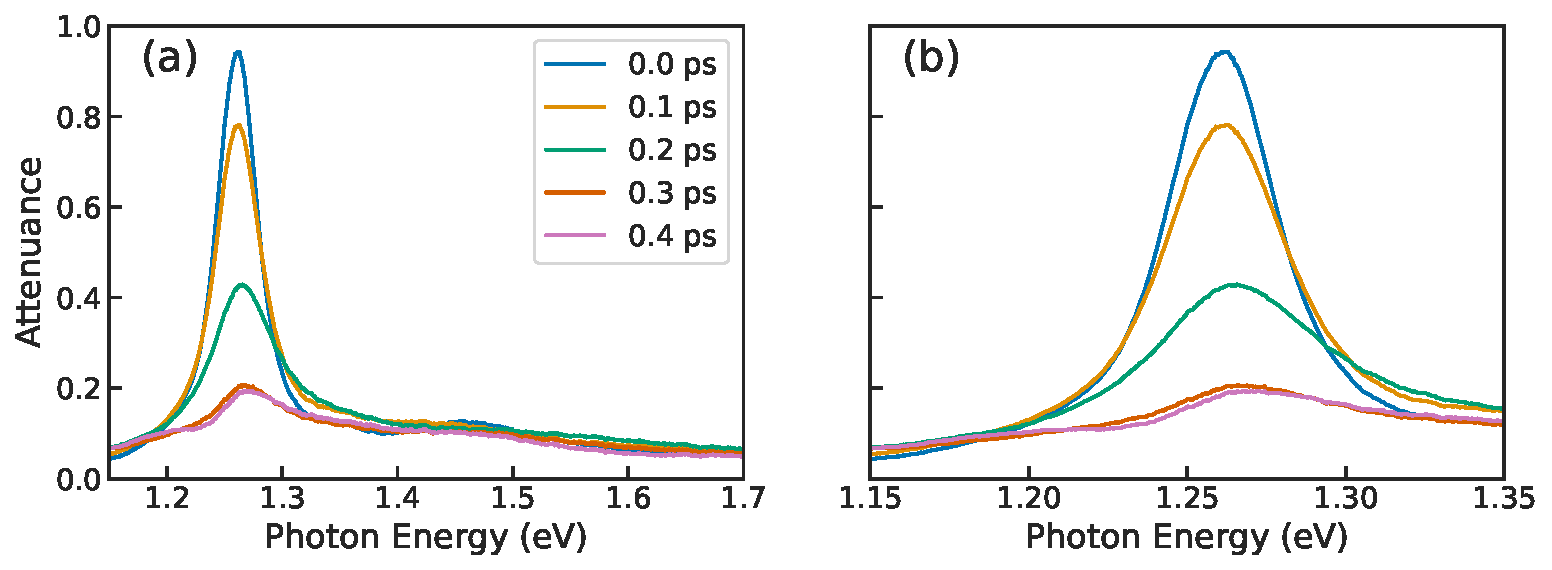
\includegraphics[height=2.4in]{images/chapter_my_data/Weilu_CNT_4mW_E11_decay} \phantomsubcaption}
	{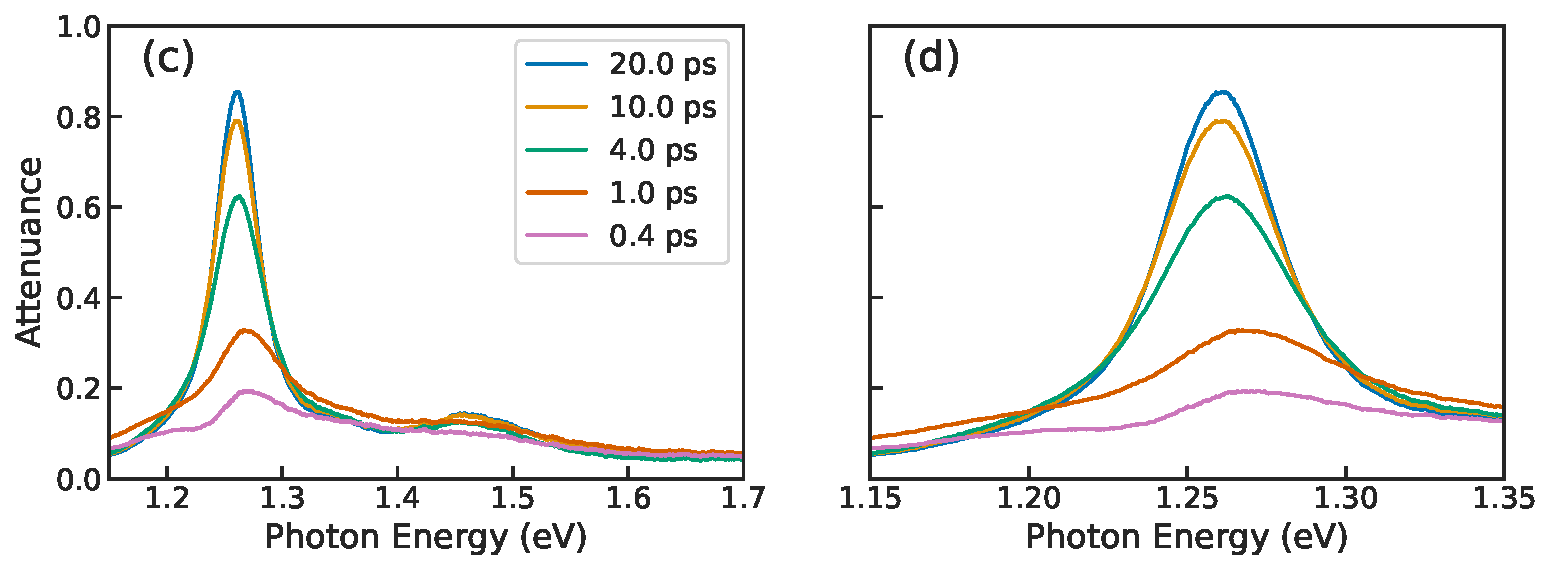
\includegraphics[height=2.4in]{images/chapter_my_data/Weilu_CNT_4mW_E11_recovery} \phantomsubcaption}
	\caption{Normalized attenuance traces measured at the indicated time delay after resonantly exciting the $E_{22}$ transition with a power density of 7.82 GW/cm$^2$. (a) Total attenuance showing the decay of the absorption at the $E_{11}$ peak at 1.26 eV as well as the attenuation of the phonon sideband located at 1.35 eV. (b) A close-up of the changes $E_{11}$ spectral region shown in Figure (a). (c) Total attenuance at later times showing the recovery of the $E_{11}$ and phonon sideband peaks. (d) A close-up of the changes $E_{11}$ spectral region shown in Figure (c).}
	\label{fig:weilu_cnt_time_traces}
\end{figure}

\begin{figure}[ht]
	\centering
	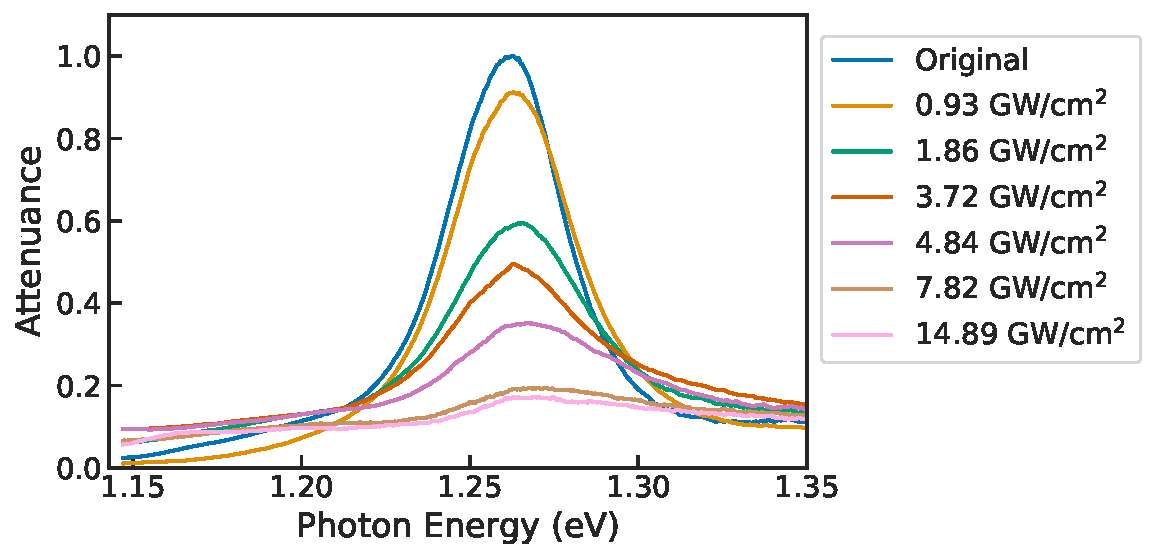
\includegraphics[height=2.4in]{images/chapter_my_data/Weilu_CNT_abs_max_change}
	\caption{Maximum decay of the $E_{11}$ peak observed at the labeled excitation power densities. The top-most trace shows the linear absorption of the spectral region. At higher power densities, the $E_{11}$ resonance diminishes more and more due to the creation of carriers. The peak also slightly blueshifts and broadens.}
	\label{fig:weilu_cnt_max_decay}
\end{figure}

\begin{figure}[H]
	\centering
	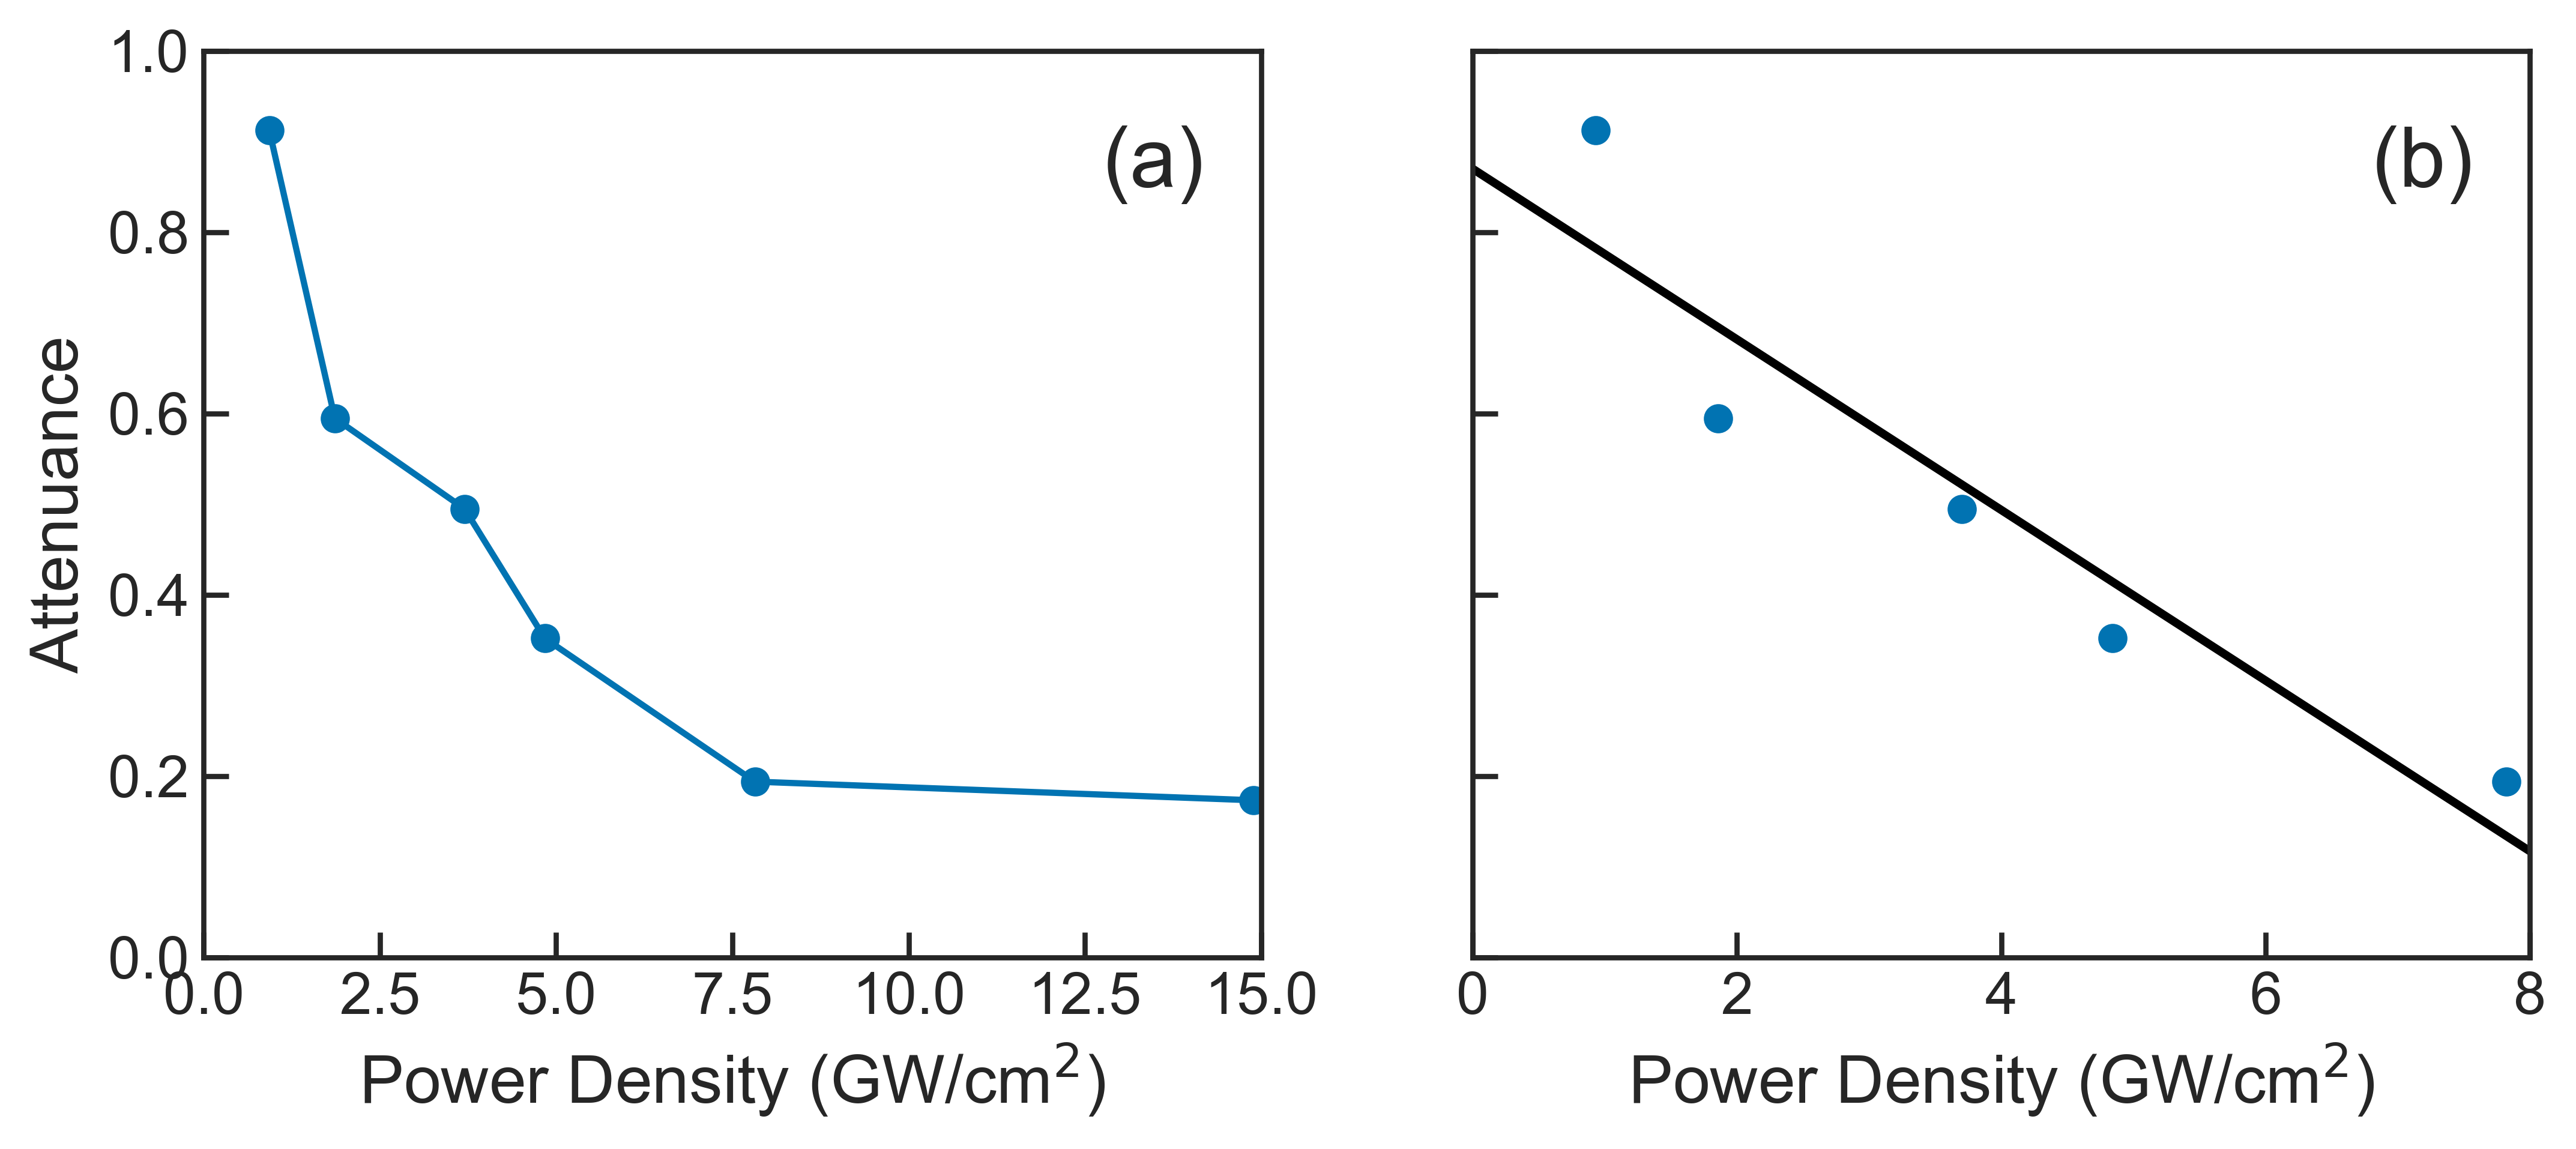
\includegraphics[height=2.4in]{images/chapter_my_data/Weilu_CNT_max_attenuance_and_fit}
	\caption{Maximum attenuance of the $E_{11}$ peak as a function of power density obtained from Figure \ref{fig:weilu_cnt_max_decay}. (a) Photo-bleaching of the $E_{11}$ resonance appears to saturate above a power density of 8 GW/cm$^2$. (b) Below power densities of 8 GW/cm$^2$, the decay of the $E_{11}$ peak is linearly proportional to the power density.}
	\label{fig:weilu_cnt_max_decay_fit}
\end{figure}

\begin{figure}[ht]
	\centering
	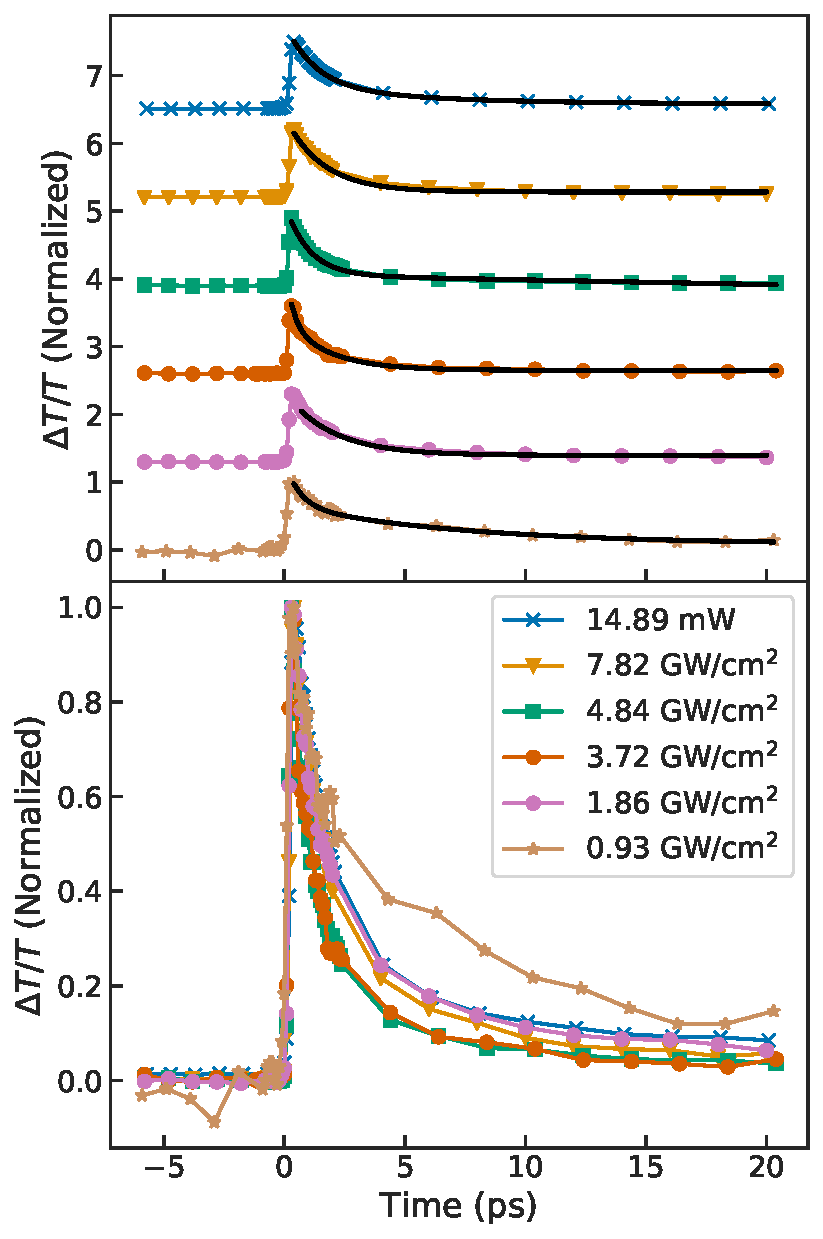
\includegraphics[height=5.4in]{images/chapter_my_data/Weilu_CNT_diff_trans_fits_and_normalized}
	\caption{ Normalized differential transmission measured at the $E_{11}$ resonance at the labeled power densities. (a) Each curve is manually offset for clarity. The solid black lines correspond to fits to the data using a bi-exponential decay model. (b) The differential transmission does not appear to have a significant dependence on the pump power density especially at higher intensities. The dynamics at the lowest intensity are dominated by the slower decay process. At higher intensities, all the measured traces do not show significant deviations from each other as expected from the effects of efficient exciton-exciton annihilation. }
	\label{fig:weilu_cnt_normalized_dt}
\end{figure}




\begin{figure}[ht]
	\centering
	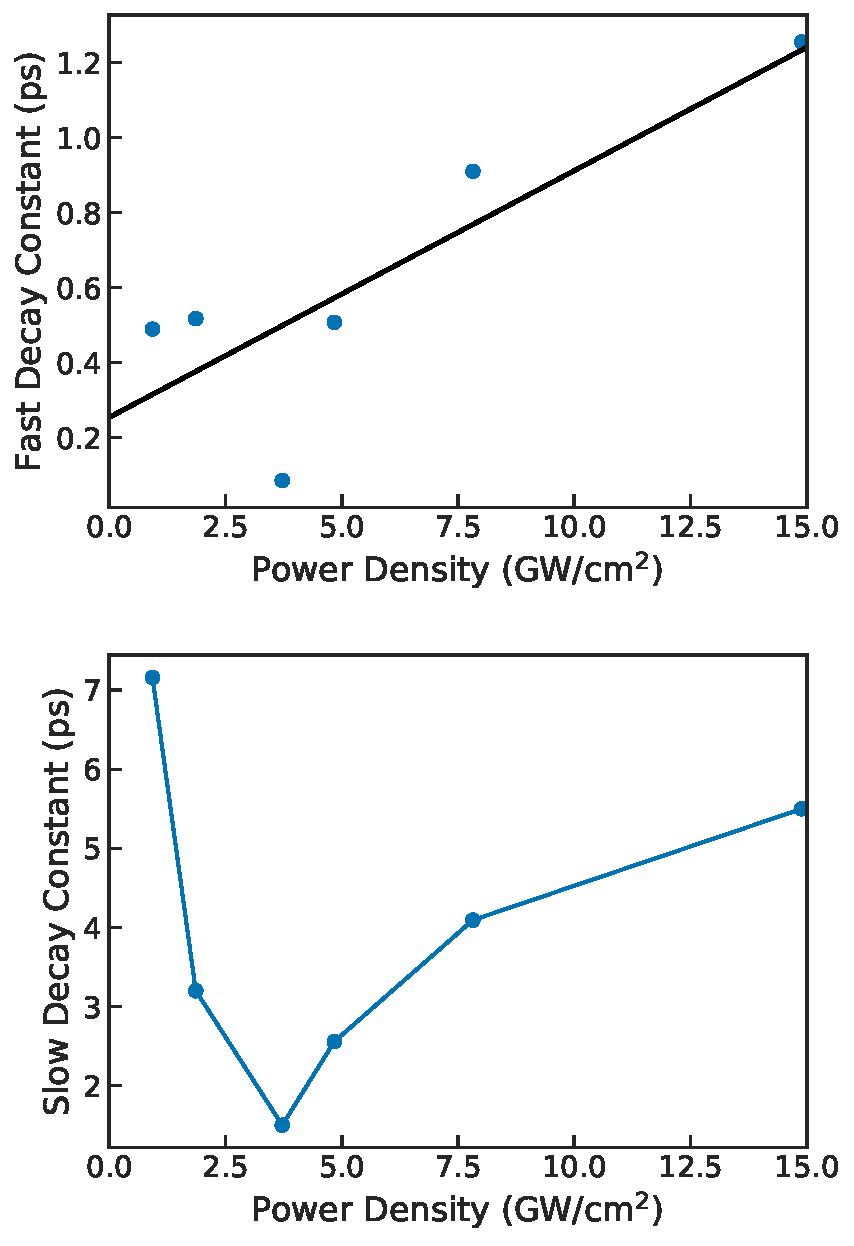
\includegraphics[height=5.4in]{images/chapter_my_data/Weilu_CNT_Fast_Slow_Decay_Const}
	\caption{(a) Fast and (b) slow decay constants extracted from the fits to the data shown in Figure \ref{fig:weilu_cnt_normalized_dt}(a). The the fast decay constant increases linearly with with the power density. This does not corroborate efficient exciton-exciton annihilation, where the fast decay constant would be expected to decrease with the power density rather than increase. The slow decay constant however shows a slightly different trend. While it appears to dominate the dynamics observed at the lower power density it decreases, it diminishes at medium intensities but increases yet again at the highest intensities.}
	\label{fig:weilu_cnt_decay_const}
\end{figure}


\clearpage
\subsection{Polymer-Wrapped (6,5)-Enriched Dispersion}



\begin{figure}[H]%
	\centering
	{\includegraphics[height=2.4in]{images/chapter_my_data/Jan_CNT_ABS_1mW_decay} \phantomsubcaption}
	{\includegraphics[height=2.4in]{images/chapter_my_data/Jan_CNT_ABS_1mW_recovery} \phantomsubcaption}
	\caption{Attenuance traces measured at the indicated time delay after resonantly exciting the $E_{22}$ transition with a power density of 1.9 GW/cm$^2$. (a) Total attenuance showing the decay of the absorption at the $E_{11}$ peak at 1.26 eV as well as the attenuation of the phonon sideband located at 1.35 eV. (b) A close-up of the changes $E_{11}$ spectral region shown in Figure (a). (c) Total attenuance at later times showing the recovery of the $E_{11}$ and phonon sideband peaks. (d) A close-up of the changes $E_{11}$ spectral region shown in Figure (c).}
	\label{fig:jan_cnt_time_traces}
\end{figure}

\begin{figure}[ht]
	\centering
	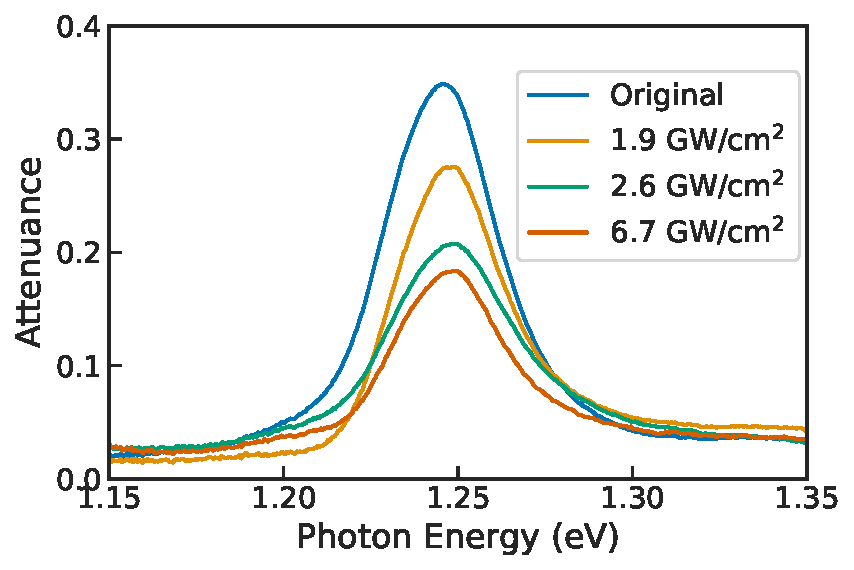
\includegraphics[height=2.4in]{images/chapter_my_data/Jan_CNT_max_abs_change}
	\caption{Maximum decay of the $E_{11}$ peak observed at the labeled excitation power densities. The top-most trace shows the linear absorption of the spectral region. At higher power densities, the $E_{11}$ resonance increasingly diminishes due to the creation of carriers.}
	\label{fig:jan_cnt_max_decay}
\end{figure}

\begin{figure}[H]
	\centering
	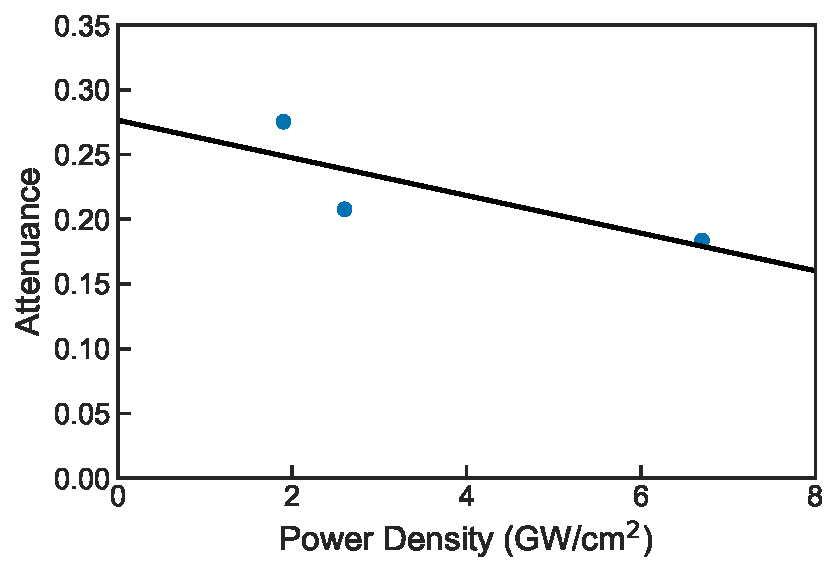
\includegraphics[height=2.4in]{images/chapter_my_data/Jan_CNT_max_attenuance_and_fit}
	\caption{Maximum attenuance of the $E_{11}$ peak as a function of power density obtained from Figure \ref{fig:jan_cnt_max_decay}. The attenuance appears to decrease with the power density in a linear fashion.}
	\label{fig:jan_cnt_max_decay_fit}
\end{figure}

\begin{figure}[ht]
	\centering
	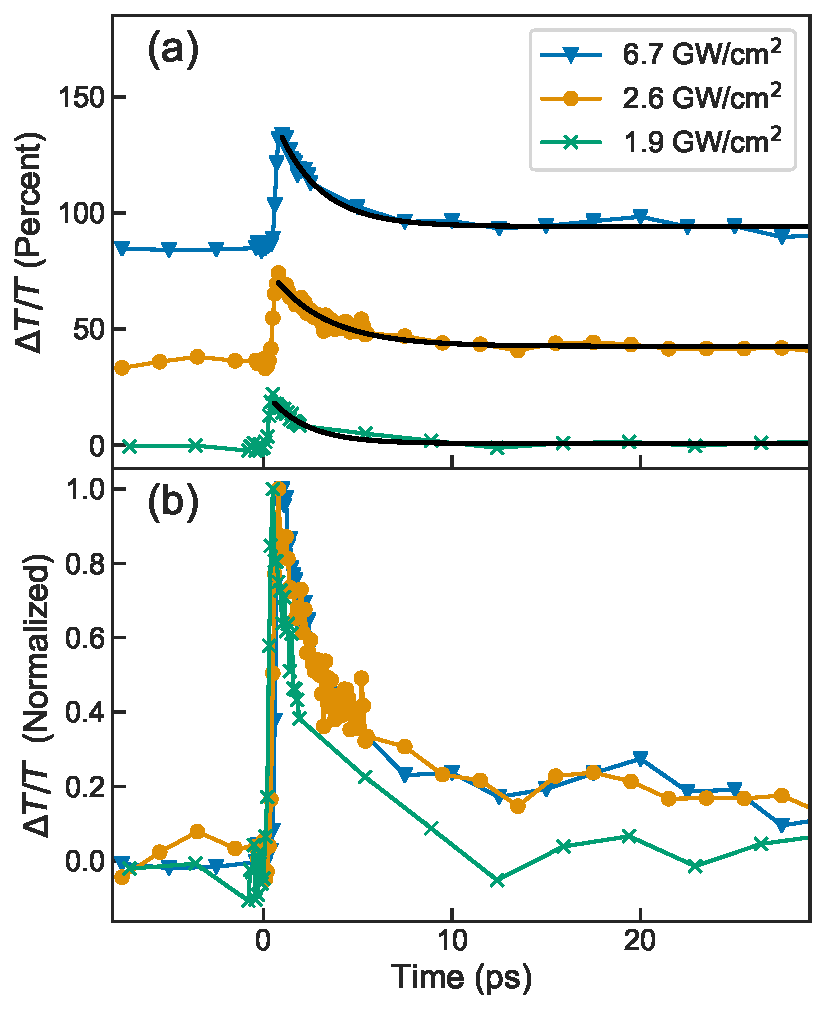
\includegraphics[height=4.4in]{images/chapter_my_data/Jan_CNT_diff_trans_fits_and_normalized}
	\caption{(a) Differential transmission measured at the $E_{11}$ resonance at the labeled power densities. Each curve is manually offset for clarity. The solid black lines correspond to fits to the data using an exponential decay model. (b) Normalized differential transmission measured at the $E_{11}$ transition. The traces do not appear to show a significant dependence on the power density of the optical pump. Furthermore, the signals measured at 2.6 GW/cm$^2$ and 6.7 GW/cm$^2$ overlap each other.}
	\label{fig:jan_cnt_max_normalized_dt}
\end{figure}

\clearpage

\begin{figure}[ht]
	\centering
	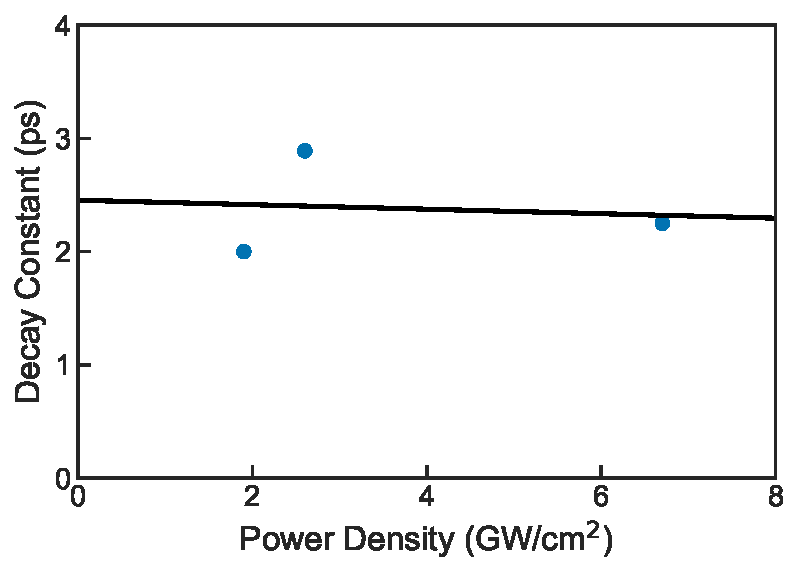
\includegraphics[height=2.5in]{images/chapter_my_data/Jan_CNT_decay_const_fit}
	\caption{Exponential decay constants obtained from Figure \ref{fig:jan_cnt_decay_const}. The decay constants do not show a significant dependence on the power density of the optical pump. }
	\label{fig:jan_cnt_decay_const}
\end{figure}

\section{Discussion}

Figures \ref{fig:weilu_cnt_time_traces} (DOC-Suspended Sample) and \ref{fig:jan_cnt_time_traces} (Polymer-Wrapped Sample) show a very fast response occuring at the $E_{11}$ resonance shortly after resonantly exciting the $E_{22}$ transition. It appears that $E_{22}$ excitons quickly decay to form $E_{11}$ excitons. This observation agrees with work of Manzoni et al (2005) who observed that inter-subband relaxation occurs on a femtosecond timescale.

The two figures also do show some key differences. In Figure \ref{fig:weilu_cnt_time_traces}, the $E_{11}$ peak broadens and blueshifts. This is typically interpreted as an indication of exciton-exciton screening \cite{shah1996ultrafast}. In the presence of a large population of excitons, the Coulomb interactions between electrons and holes become screened. This leads to a reduced binding energy and broadening of $E_{11}$ peak due to the lower stability of excitons. These results differ from the observations by Ostojic et al.\ (2005) as well as Murakami and Kono (2009) who did not observe any change in the positions and linewidths of the optical resonances in their samples.

If exciton-exciton annihilation were indeed efficient, then the significant photo-bleaching of the optical resonances in SWCNTs should not at all be possible as mentioned by Murakami and Kono (2009). Furthermore, the strong attenuation of oscillator strength of the $E_{11}$ peak may suggest that the density of photo-generated excitons exceeds the Mott density of the system. Excitons, being composed of two half-integer spin quasiparticles, are expected to behave as bosons \cite{Ashcroft, laikhtman2007excitons}. Hence, there should not be photo-bleaching of resonance if only excitons are created by the optical pump as bosons are exempt from the Pauli exclusion principle. The results here suggest that Fermions also play a role in the observed carrier dynamics.

Unlike Figure \ref{fig:weilu_cnt_time_traces}, Figure \ref{fig:jan_cnt_time_traces} instead shows a narrowing of the $E_{11}$ resonance, especially on the lower energy region of the $E_{11}$ resonance. This could be a sign of spectral-hole burning. Here, the $E_{11}$ peak is inhomogenously broadened as the dispersion contains an ensemble of (6,5) SWCNTs. As a result the homogenous optical resonances, emerging from individual nanotubes, in the lower energy region of the $E_{11}$ resonance will be the first to become photo-bleached.

Figures \ref{fig:weilu_cnt_max_decay}  (DOC-Suspended Sample) and \ref{fig:jan_cnt_max_decay} (Polymer-Wrapped Sample) show the decay of the $E_{11}$ peak as the power density of the optical pump is increased. In the case of Figure \ref{fig:weilu_cnt_max_decay}, the $E_{11}$ peak almost completely disappears, whereas in Figure \ref{fig:jan_cnt_max_decay}, the limited data does seem to indicate saturation behavior as the change from 2.9 to 6.7 GW/cm$^2$ is almost negligible when compared to the change from 1.9 to 2.6 GW/cm$^2$. The maximum attenuances from these figures are plotted in Figures \ref{fig:weilu_cnt_max_decay_fit} and \ref{fig:jan_cnt_max_decay_fit} respectively. Both figures show that the oscillator strength of the $E_{11}$ peak decreases as the pump intensity increases. Figure \ref{fig:weilu_cnt_max_decay_fit} shows a linear decrease that occurs up until a power density of 7.8 GW/cm$^2$. After that point, the decrease in the attenuance begins to saturate. Due to the limited data collected in Figure \ref{fig:jan_cnt_max_decay_fit} it is more difficult to conclude whether saturation does occur. However, the decrease in the attenuance appears to be somewhat linear as shown by the linear fit to the data.

The changes in differential transmission recorded at the $E_{11}$ resonance do not corroborate the previously reported evidence of efficient exciton-exciton annihilation. Figures \ref{fig:weilu_cnt_normalized_dt} (DOC-Suspended Sample) and \ref{fig:jan_cnt_max_normalized_dt} (Polymer-Wrapped Sample) demonstrate this. In Figure \ref{fig:weilu_cnt_normalized_dt}(a), DOC suspension sample showed carrier dynamics that agree with a bi-exponential fit whereas, those of polymer-wrapped sample shown in Figure \ref{fig:jan_cnt_max_normalized_dt} instead correspond to exponential decays. This suggests that carrier relaxation in the polymer-wrapped sample occurs more slowly. Overall, the normalized differential transmission data measured at the indicated power densities closely overlap one another and a fast initial decay does not dominate the observed dynamics at higher power densities. This result however may not be too surprising as previous transient absorption measurements in the literature also did not observe any nonlinear carrier dynamics associated with efficient exciton-exciton annihilation \cite{ostojic2004interband, manzoni2005intersubband, ma2005femtosecond, luer2009size}.

Furthermore, the scenario presented by dominant exciton-exciton annihilation processes suggests that the initial decay should become faster with increasing power density. The decay constants extracted from the differential transmission data do not exhibit such a trend. Figures \ref{fig:weilu_cnt_decay_const} and \ref{fig:jan_cnt_decay_const} show the extracted decay constants obtained by fitting to the differential transmission measured in each sample respectively. In Figure \ref{fig:weilu_cnt_decay_const}(a), the fast decay constant increases linearly with the power density, whereas in Figure \ref{fig:jan_cnt_decay_const} the decay time does not change significantly.


\section{Conclusions}

In this work, we studied the carrier relaxation dynamics of two ensembles of SWCNTs induced by resonant $E_{22}$ excitation. These two ensembles included SWCNTs disperesed in an aqueous solution using DOC as a surfactant as well as another dispersion of polymer-wrapped SWCNTs dispersed in toluene. In both samples, we observed a fast response at the $E_{11}$ transition after creating $E_{22}$ excitons with the optical pump. In the DOC suspension, the $E_{11}$ peak broadened, blueshifted and was almost completely photo-bleached, suggesting that enough carriers were created to exceed the Mott density. However, in the polymer-wrapped sample, the significant photo-bleaching of the lower energy region of the $E_{11}$ was interpreted as a signature of spectral hole burning.

In addition, the data do not show signs of efficient exciton-exciton annihilation. For the samples studied, the measurements indicate that the dominance of a fast exponential is rather weak and does not appropriately scale with the fluence of the optical pump as expected by time-resolved photoluminenscence measurements. Instead of an intial decay that becomes faster with higher pump intensities, a signature of exciton-exciton annihilation, we observed an intial decay that either slows down with increasing pump intensity or remains roughly constant depending on the sample being studied. In conclusion, the narrative of efficient exciton-exciton may be not be completely conclusive and warrants further study.
